\documentclass[tikz,border=8pt]{standalone}
\usepackage{amsmath}
\usetikzlibrary{arrows.meta,calc}

\definecolor{ink}{HTML}{21352F}
\definecolor{teal}{HTML}{087F7B}
\definecolor{blue}{HTML}{4B77A8}
\definecolor{gold}{HTML}{C58B2A}
\definecolor{rose}{HTML}{B65A62}

\begin{document}
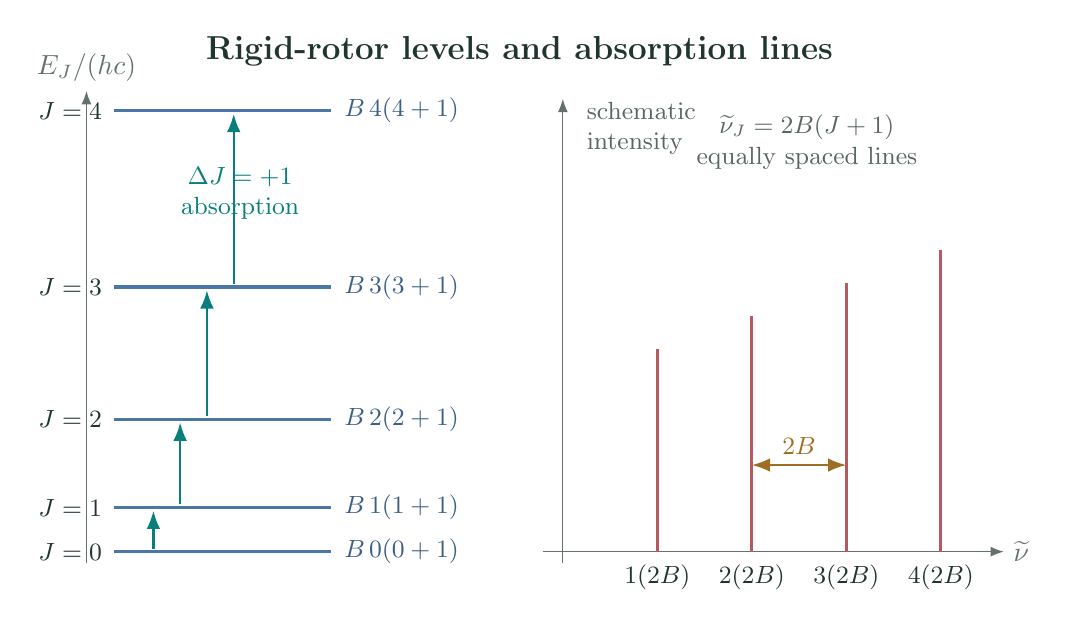
\begin{tikzpicture}[font=\sffamily,text=ink,>=Latex]
  \node[font=\bfseries\large] at (0,6.35)
    {Rigid-rotor levels and absorption lines};

  \draw[->,ink!70] (-5.5,-.15)--(-5.5,5.85)
    node[above] {$E_J/(hc)$};

  \foreach \J in {0,...,4}{
    \pgfmathsetmacro{\yy}{0.28*\J*(\J+1)}
    \draw[blue,very thick] (-5.15,\yy)--(-2.4,\yy);
    \node[left,font=\small] at (-5.18,\yy) {$J=\J$};
    \node[right,font=\small,text=blue!80!black] at (-2.35,\yy)
      {$B\,\J(\J+1)$};
  }

  \foreach \J in {0,...,3}{
    \pgfmathtruncatemacro{\K}{\J+1}
    \pgfmathsetmacro{\ya}{0.28*\J*(\J+1)}
    \pgfmathsetmacro{\yb}{0.28*\K*(\K+1)}
    \draw[teal,thick,->]
      ({-4.65+0.34*\J},\ya+0.04)--
      ({-4.65+0.34*\J},\yb-0.04);
  }
  \node[teal,font=\small,align=center] at (-3.55,4.55)
    {$\Delta J=+1$\\absorption};

  \draw[->,ink!70] (.3,0)--(6.15,0)
    node[right] {$\widetilde\nu$};
  \draw[->,ink!70] (.55,-.15)--(.55,5.75);
  \node[font=\small,align=left,anchor=west,text=ink!75]
    at (.73,5.38) {schematic\\intensity};

  \foreach \n in {1,...,4}{
    \pgfmathsetmacro{\xx}{0.55+1.20*\n}
    \pgfmathsetmacro{\hh}{2.15+0.42*\n}
    \draw[rose,very thick] (\xx,0)--(\xx,\hh);
    \node[below,font=\small] at (\xx,-.04) {$\n(2B)$};
  }

  \draw[<->,gold!80!black,thick]
    (2.95,1.1)--(4.15,1.1)
    node[midway,above,font=\small] {$2B$};
  \node[align=center,font=\small,text=ink!75] at (3.65,5.2)
    {$\widetilde\nu_J=2B(J+1)$\\equally spaced lines};
\end{tikzpicture}
\end{document}
